\documentclass[11pt, spanish]{report}
\usepackage[spanish]{babel}
\usepackage[utf8]{inputenc}
\usepackage{geometry}
\usepackage{graphicx}
 \geometry{
 a4paper,
 total={170mm,257mm},
 left=20mm,
 top=20mm,
 }
\usepackage{graphicx}
\graphicspath{ {images/} }
\usepackage[utf8]{inputenc}
\decimalpoint
\title{Actividad 6: Modelo INIFAP-CECH}
\author{César Andrés Pérez Robinson }
\date{Marzo 2019}

\begin{document}

\maketitle

\section{Introducción}
En este reporte se muestra el código y descripción utilizado en jupyter notebook para comparar el modelo de Utah y el modelo INIFAP-CECH. Ambos se utilizan para estimar el fin de la dormancia invernal en los árboles frutales.\\
El modelo de Utah no se adapta a zonas de inviernos débiles como es el caso de las zonas agrícolas del Estado de Sonora. A partir de esto, el Instituto de Investigaciones Forestales, Agrícolas y Pecuarias (INIFAP), desarrolla su propio modelo adecuandolo.
\section{Código utilizado}
De manera inicial, se descargan los progamas a utilizar
\begin{verbatim}
    import pandas as pd
    import numpy as np
\end{verbatim}
Se descargan los datos en un dataframe
\begin{verbatim}
    df = pd.read_csv("vid18_180219.dat",delimiter=',')
\end{verbatim}
Se seleccionan las columnas de interés y se observan los primeros cinco datos.
\begin{verbatim}
    [IN]
    df = df.filter(['TIMESTAMP','AirTC_Avg'],axis=1)
    df.head()
    
    [OUT]
    TIMESTAMP	            AirTC_Avg
0	2018-05-11 20:10:00	    23.50
1	2018-05-11 20:20:00	    22.96
2	2018-05-11 20:30:00	    22.73
3	2018-05-11 20:40:00	    22.40
4	2018-05-11 20:50:00	    22.46
\end{verbatim}
Se hace que la variable TIMESTAMP sea presentada en formato de fecha y se crean las columnas de año, mes, día y hora.
\begin{verbatim}
    df['TIMESTAMP'] = pd.to_datetime(df.apply(lambda x: x['TIMESTAMP'],1), 
    dayfirst=True)
    df['Año']=df['TIMESTAMP'].dt.year
    df['Mes']=df['TIMESTAMP'].dt.month
    df['Dia']=df['TIMESTAMP'].dt.day
    df['Hora']=df['TIMESTAMP'].dt.hour 
\end{verbatim}
Se toman los datos desde el primero de Noviembre del 2018 usando.
\begin{verbatim}
    [IN]
    df = df[(df['TIMESTAMP'] >= "2018-11-1")]
    df= df.reset_index(drop=True)
    df.head()
    
    [OUT]
    TIMESTAMP	           AirTC_Avg    Año 	Mes	Dia	Hora	TempProm
    0	2018-11-01 00:00:00     9.13    2018	11	1   0       9.13
    1	2018-11-01 00:10:00     8.89    2018	11	1   0       8.89
    2	2018-11-01 00:20:00     8.66    2018	11	1   0       8.66
    3	2018-11-01 00:30:00     8.52    2018	11	1   0       8.52
    4	2018-11-01 00:40:00     8.47    2018	11	1   0       8.47
\end{verbatim}
Se agrega una columna duplicada de AirTC\_Avg y la elimino junto con TIMESTAMP.
\begin{verbatim}
    [IN]
    df['TempProm'] = df['AirTC_Avg']
    df=df.drop(['TIMESTAMP','AirTC_Avg'],1)
    df.head()
    
    [OUT]
        Año     Mes	Dia	Hora	TempProm
    0   2018    11  1   0   	9.13
    1   2018    11  1   0   	8.89
    2   2018    11  1   0   	8.66
    3   2018    11  1   0   	8.52
    4   2018    11  1   0   	8.47
\end{verbatim}
Se crean las columnas de TMAX y TMIN y se quitan los años repetidos por hora.
\begin{verbatim}
    [IN]
    df["TMAX"] = np.round(df.groupby(["Año","Mes","Dia"])["TempProm"].transform("max"),decimals=1)
    df["TMIN"] = np.round(df.groupby(["Año","Mes","Dia"])["TempProm"].transform("min"),decimals=1)
    df = df.drop_duplicates(subset=["Año","Mes","Dia","Hora"])
    df=df.reset_index(drop=True)
    df.head(10)
    
    [OUT]
    Año     Mes	Dia Hora	TempProm	    TMAX	    TMIN
0   2018    11  1   0       9.130	    29.6	    6.1
1   2018    11  1   1       8.560	    29.6	    6.1
2   2018    11  1   2       8.830	    29.6	    6.1
3   2018    11  1   3       9.130	    29.6	    6.1
4   2018    11  1   4       7.924	    29.6	    6.1
5   2018    11  1   5       7.261	    29.6	    6.1
6   2018    11  1   6       7.723	    29.6	    6.1
7   2018    11  1   7       6.125	    29.6	    6.1
8   2018    11  1   8       12.430	    29.6	    6.1
9   2018    11  1   9       18.080	    29.6	    6.1
\end{verbatim}
Se crea un loop utilizando el Modelo de Richardson.
\begin{verbatim}
    URichardson = []
for i in range(0, len(df)):
    temp = df.TempProm[i]
    if (temp <= 1.4):
        temp = 0
        URichardson.append(temp)
    if (1.4 < temp <= 2.4):
        temp = 0.5
        URichardson.append(temp)
    if (2.4 < temp and temp <= 9.1):
        temp = 1.0
        URichardson.append(temp)
    if (9.1 < temp and temp <= 12.4):
        temp = 0.5
        URichardson.append(temp)
    if (12.4 < temp and temp <= 15.9):
        temp = 0
        URichardson.append(temp)
    if (15.9 < temp and temp <= 18.0):
        temp = -0.5
        URichardson.append(temp)
    if (18.0 < temp):
        temp = -1.0
        URichardson.append(temp)
\end{verbatim}
Utilizando elm odelo de INIFAP-CECH, donde HF = el número de horas frío por día (0 < T <= 10ºC) y HFE = El número de horas frío efectivas por día ( HFE= HF - número de horas con T >= 25ºC). Primero se tienen que crear los arreglos necesarios.
\begin{verbatim}
    AHF = []
for i in range(0,len(df)):
    thf = df['TempProm'][i]
    if(0 < thf and thf <= 10):
        AHF.append(1)
    else:
        AHF.append(0)
AHC = []
for i in range(0,len(df)):
    thc = df['TempProm'][i]
    if (thc >= 25):
        AHC.append(1)
    else:
        AHC.append(0)
\end{verbatim}
Se agregan los valores a nuestro dataframe.
\begin{verbatim}
    [IN]
    df['Modelo UR']=URichardson
    df['aHF']=AHF
    df['aHC']=AHC
    df.head()
    
    [OUT]
        Año     Mes	Dia	Hora	TempProm	TMAX	TMIN	ModeloUR	HF	HC	aHF	aHC
    0	2018        11	1   	0	    9.130	29.6	  6.1	    0.5	 1	 0	 1	  0
    1	2018        11	1   	1	    8.560	29.6	  6.1	    1.0	 1	 0	 1	  0
    2	2018        11	1   	2	    8.830	29.6	  6.1	    1.0	 1	 0	 1	  0
    3	2018        11	1   	3	    9.130	29.6	  6.1	    0.5	 1	 0	 1	  0
    4	2018        11	1   	4	    7.924	29.6	  6.1	    1.0	 1	 0	 1	  0
\end{verbatim}
Para contar cuantos valores se obtienen por día sobre el modelo UR, HF y HC.
\begin{verbatim}
    df["UF24"] = df.groupby(["Año","Mes","Dia"])["Modelo UR"].transform("sum")
    df["HF"] = df.groupby(["Año","Mes","Dia"])["aHF"].transform("sum")
    df["HC"] = df.groupby(["Año","Mes","Dia"])["aHC"].transform("sum")
    
    df = df.drop(["aHF",'aHC','Modelo UR'], 1)
\end{verbatim}
Realizando de nuevo los datos repetidos por hora.
\begin{verbatim}
    df = df.drop_duplicates(subset=["Año","Mes","Dia"])
    df=df.reset_index(drop=True)
\end{verbatim}
Obteniendo el valor acumulado para UF24 y HFE = el número de horas frío efectivas por día (HFE = HF - número de horas con T mayor o igual a 25ºC.
\begin{verbatim}
    [IN]
    df['HFE']=df.HF-df.HC
    
    [OUT]
    
    Año  Mes Dia HorA  TempProm   TMAX    TMIN    HF  HC    UF24
0   2018	11  	1 	 0      9.13	    29.6    6.1	    8   5     -2.5
1   2018	11  	2 	 0	    10.79	    31.4    10.0    0   7     -9.5
2   2018	11  	3 	 0	    12.85	    30.5    10.2    0   8     -8.5
3   2018	11  	4 	 0	    13.14	    31.4    11.2    0   8     -11.0
4   2018	11  	5 	 0	    14.41	    31.2    11.1    0   7     -8.5
\end{verbatim}
Para graficar ambos modelos. Se muestra en la Figura 1.
\begin{verbatim}
    import matplotlib.pyplot as plt

y1 = [df['HFE'][i] for i in range(0,len(df))]
y2 = [df['UF24'][i] for i in range(0,len(df))]


plt.figure(figsize=(9,5))
plt.plot(y1, label = "HFE", color = 'Blue')   
plt.plot(y2, label = "UF24", color = 'Green')   
plt.xlabel("Días")   
plt.ylabel("Modelos")  
plt.legend()
plt.grid()
plt.title('HFE y UF24.')
plt.show()
\end{verbatim}
\begin{figure}[ht]
\caption{Comparación de ambos modelos}
\centering
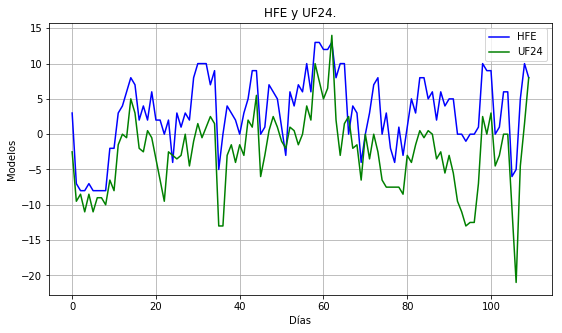
\includegraphics[width=0.65\textwidth]{HFEyUF24.png}
\end{figure}
Y por último, se grafican los datos de cada modelo de manera acumulada en la Figura 2, utilizando.
\begin{verbatim}
    y1 = df['HFE'].cumsum()
    y2 = df['UF24'].cumsum()

plt.figure(figsize=(9,5))
plt.plot(y1, label = "HFE", color = 'Blue')   
plt.plot(y2, label = "UF24", color = 'Green')   
plt.xlabel("Días")   
plt.ylabel("Modelos")  
plt.legend()
plt.grid()
plt.title('Acumulados de HFE y UF24.')
plt.show()
\end{verbatim}
\begin{figure}[ht]
\caption{Datos acumulados de ambos modelos}
\centering
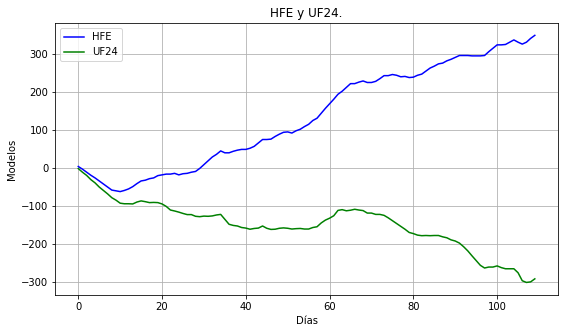
\includegraphics[width=0.65\textwidth]{acum.png}
\end{figure}
\end{document}
